% Provenance (never printed): see sources/outline_sources.md (Year 2: anatexis, migmatites,
% granite types and their sources). Wet granite solidus from Stern and Wyllie (1981) and
% Boettcher and Wyllie (1968); dehydration-melting brackets from Patino Douce and Harris
% (1998), Berger and Kalt (1999), Skjerlie and Johnston (1996); water solubility from Holtz
% et al. (1995); migmatite terms from the IUGS-SCMR proposal and BGS RR 99-02; aluminosity
% after Shand (as given by Moyen et al. 2017); figure data in figdata/bachelor-2/anatexis.py
% (paths from ptpaths.py); exercise and problem values in the Book 4 scratch calculator
% calc/ch12.py.
\chapter{Smelten van de korst: migmatieten en granieten}\label{ch:b2:crustal-melting}

Graniet maakt de continenten licht, en de mantel kan het niet rechtstreeks maken: de
smelten van \omterm{def:b2:mantle-melting:peridotites}{peridotiet} zijn basalten. Het meeste graniet is continentale korst die zichzelf doet smelten.
Wanneer een verdikte gebergtewortel opwarmt, wanneer basalt zich onder de korst ophoopt, of wanneer een heet
gesteente opstijgt en zijn druk daalt, staan de mica's en amfibolen van de diepe korst hun
water af, verschijnt er een granitische vloeistof tussen de korrels, en wordt het gesteente een
\omterm{def:b2:crustal-melting:migmatite}{migmatiet}, half metamorf, half magmatisch. Dit hoofdstuk volgt die vloeistof van haar eerste
filmpjes tot de \omterm{def:b2:magma-emplacement:bodies}{pluton} die ze kan opbouwen, en leest in de chemie van een graniet het gesteente waaruit ze
kwam.

\begin{recall}
\textbf{Uit Boek~2}: graniet, granitoïde en granodioriet; felsische en mafische
gesteenten; de wortels van gebergtegordels. \textbf{Uit Boek~3}: de radiogene
warmteproductie in de korst; de hydrolyse van silicaten en kleimineralen. \textbf{Uit de scheikundeboeken}: de solidus en de liquidus
van een binair systeem, molaire massa en stofhoeveelheid. \textbf{Uit
\cref{ch:b2:magma-emplacement}}: \omterm{def:b2:magma-emplacement:bodies}{gangen}, \omterm{def:b2:magma-emplacement:bodies}{plutons} en \omterm{def:b2:magma-emplacement:ascent}{diapieren}. \textbf{Uit
\cref{ch:b2:mantle-melting}}: \omterm{def:b2:mantle-melting:melting}{partieel smelten}, \omterm{def:b2:mantle-melting:peritectic}{incongruent smelten} en
\omterm{def:b2:mantle-melting:melting}{decompressiesmelten}. \textbf{Uit \cref{ch:b2:metamorphic-facies}}: \omterm{def:b2:metamorphic-facies:protoliths}{metapelieten}, de \omterm{def:b2:metamorphic-facies:clapeyron}{Clapeyronhelling} van
een reactie en de facies. \textbf{Uit \cref{ch:b2:pt-paths}}: \omterm{def:b2:pt-paths:ptt}{P--T--t-paden} en het
verdikkingsmodel van de korst.
\end{recall}

\section{Waarom de korst smelt}\label{sec:b2:crustal-melting:why}

Het woord ervoor is oud en eenvoudig.

\begin{definition}[Anatexis]\label{def:b2:crustal-melting:anatexis}
\emph{Anatexis}\index{anatexis} is het smelten van een gesteente, wat de smeltgraad ook is;
in de praktijk wordt het woord gebruikt voor het \omterm{def:b2:mantle-melting:melting}{partieel smelten} van de continentale korst.
\end{definition}
% ledger: scmr:migmatite

\subsection*{De natte solidus}

Graniet smelt alleen bij een lage temperatuur als het nat is. Stern en Wyllie lieten een
biotietgraniet uit de \omterm{def:b2:magma-emplacement:bodies}{batholiet} van de Sierra Nevada smelten met een overmaat water: de eerste vloeistof verscheen bij
\qty{680}{\celsius} bij \qty{2}{kbar} en bij \qty{620}{\celsius} bij \qty{10}{kbar}, en het
hele gesteente was bij \qty{2}{kbar} al gesmolten op slechts \qty{35}{\celsius} boven de solidus, maar
bij \qty{10}{kbar} pas \qty{105}{\celsius} erboven. Hetzelfde graniet, eerder bestudeerd door
Boettcher en Wyllie, begon te smelten bij \qty{605}{\celsius} bij \qty{15.3}{kbar}; rond
\qty{17}{kbar} viel zijn plagioklaas uiteen in jadeïet en kwarts, en vanaf daar boog de solidus
weer omhoog, tot \qty{670}{\celsius} bij \qty{27}{kbar}.
% ledger: sw81:wet-solidus, bw68:wet-solidus

De natte solidus daalt naarmate de druk stijgt, het omgekeerde van een droge solidus. De reden is waar
het water heen gaat. Vrij water is een fluïdum met lage dichtheid; opgelost in de smelt neemt het heel
weinig plaats in: Holtz en collega's vonden zijn partieel molair volume in een granitische smelt dicht
bij \qtyrange{10}{12}{\cubic\centi\metre\per\mole}, tegen \qty{18}{\cubic\centi\metre\per\mole}
voor vloeibaar water bij kamertemperatuur en meer voor een heet fluïdum. De smeltreactie
\[\text{kwarts} + \text{veldspaten} + \ce{H2O}\ (\text{fluïdum}) \longrightarrow
\text{waterhoudende smelt}\]
heeft daarom een negatieve volumeverandering, terwijl haar entropieverandering, zoals bij elk smelten,
positief is: volgens de betrekking van Clapeyron uit \cref{ch:b2:metamorphic-facies} is haar helling
$\mathrm{d}P/\mathrm{d}T = \Delta S/\Delta V$ negatief. Druk laat ook meer water
in de smelt toe: voor een haplogranietsmelt bij \qty{800}{\celsius} stijgt het verzadigingsgehalte
van \qty{2.80}{\percent} massa bij \qty{0.5}{kbar} tot \qty{9.97}{\percent} bij
\qty{5}{kbar} en \qty{13.82}{\percent} bij \qty{8}{kbar}, ongeveer \qty{1.27}{\percent} meer
per kilobar tussen 3 en \qty{8}{kbar}.
% ledger: holtz95:solubility

\begin{omfigure}
\centering
\begin{tikzpicture}
\begin{axis}[omrecord, width=0.5\linewidth, height=4.8cm,
  xmin=0, xmax=9, ymin=0, ymax=15, xlabel={$P$ (\unit{kbar})},
  ylabel={\ce{H2O} in smelt (\unit{\percent})},
  tick label style={font=\scriptsize}, label style={font=\small}]
\addplot[only marks, mark=*, mark size=1.6pt, blue!70!black]
  table[x=P_kbar, y=H2O_wt] {figdata/out/bachelor-2-anatexis-water.dat};
\addplot[thick, red!75!black] table[x=P_kbar, y=H2O_wt] {figdata/out/bachelor-2-anatexis-waterfit.dat};
\end{axis}
\end{tikzpicture}
\par\smallskip{\small Water dat een haplogranietsmelt kan oplossen bij \qty{800}{\celsius}
(gemeten punten); rood: de kleinstekwadratenlijn door de punten van 3 tot
\qty{8}{kbar}, helling \qty{1.26}{\percent} per kilobar.}
\end{omfigure}
% ledger: holtz95:solubility

Maar de diepe korst bevat weinig vrij water: een metamorf gesteente dat is verhit, heeft het meeste
van zijn poriewater al uitgedreven, via de dehydratatiereacties van
\cref{ch:b2:metamorphic-facies}. Zijn water zit nu vast in mica's en amfibolen. Het smelten
moet dan wachten tot deze mineralen zelf uiteenvallen.

\begin{definition}[Smelten met fluïdum en dehydratatiesmelten]\label{def:b2:crustal-melting:reactions}
\emph{Smelten met fluïdum}\index{smelten met fluïdum} (of door water aangedreven smelten) is
smelten in aanwezigheid van een vrij waterig fluïdum, bij of dicht bij de natte solidus; de geproduceerde
smelt wordt begrensd door de aanvoer van fluïdum. \emph{Dehydratatiesmelten}\index{dehydratatiesmelten}
(smelten zonder fluïdum) is het \omterm{def:b2:mantle-melting:peritectic}{incongruente smelten} van een waterhoudend mineraal, mica of
amfibool, met kwarts en veldspaat, zonder enig vrij fluïdum: het water van het mineraal
gaat in de smelt, en nieuwe watervrije mineralen (peritectisch kaliveldspaat, aluminiumsilicaat,
granaat, cordieriet, orthopyroxeen) groeien ernaast.
\end{definition}
% ledger: pj98:productivity, koester02:melting, pdh98:himalaya

Experimenten leggen vast waar elk waterhoudend mineraal het opgeeft. In muscovietschisten uit de
Himalaya vonden Patiño Douce en Harris dat het \omterm{def:b2:crustal-melting:reactions}{dehydratatiesmelten} begon bij 750 tot
\qty{800}{\celsius} tussen 6 en \qty{10}{kbar}; water toegevoegd aan dezelfde gesteenten verlaagde de
solidus maar gaf trondhjemitische smelten, anders dan de \omterm{def:b2:crustal-melting:leucogranite}{leucogranieten}. Een semipelitische gneis
begon te smelten rond \qty{700}{\celsius} via zijn fengitische muscoviet, maar leverde minder
dan \qty{9}{\percent} smelt op; boven \qty{800}{\celsius} gaf het uiteenvallen van biotiet en
cordieriet 10 tot \qty{63}{\percent} volume. \omterm{def:b2:crustal-melting:reactions}{Dehydratatiesmelten} van biotiet vond plaats
bij 800 tot \qty{850}{\celsius} en 0.5 tot \qty{0.7}{GPa} in de \omterm{def:b2:crustal-melting:migmatite}{migmatieten} van het
Beierse Woud, en amfibool voegt ongeveer \qty{25}{\percent} smelt in volume toe tussen 875
en \qty{925}{\celsius} bij 10 tot \qty{12.5}{kbar}. De volgorde is die van de greep op het water:
muscoviet eerst, biotiet daarna, amfibool als laatste.
% ledger: pdh98:himalaya, koester02:melting, bk99:migmatites, sj96:amphibole, moyen17:aluminosity

\begin{proposition}[Een door water begrensde smeltfractie]\label{prop:b2:crustal-melting:water}
Als bij \omterm{def:b2:crustal-melting:reactions}{dehydratatiesmelten} zonder enig vrij fluïdum een gesteente een massafractie $X$ bevat van een
waterhoudend mineraal met een massafractie $w$ water, en als al dit water in een
smelt gaat die een massafractie $c$ water bevat, dan is de massafractie smelt
\[F = \frac{X\,w}{c}.\]
Omdat $c$ niet groter kan zijn dan het verzadigingsgehalte $c_{\mathrm{sat}}$ bij de druk en
temperatuur van het smelten, geldt $F \ge X\,w/c_{\mathrm{sat}}$: hoe minder water de smelt bevat, des te
meer smelt dezelfde mica maakt.
\end{proposition}

\begin{proof}
Per kilogram gesteente geeft het mineraal $X\,w$ kilogram water af. Zonder fluïde fase
en zonder water dat in de vaste stoffen achterblijft, zit het allemaal in de smelt, waarvan de massa $F$ $c\,F$
kilogram water bevat: $c\,F = X\,w$. Omdat $c \le c_{\mathrm{sat}}$, geldt $F = Xw/c \ge
Xw/c_{\mathrm{sat}}$.
\end{proof}

Een muscoviet, \ce{KAl3Si3O10(OH)2} met molaire massa \qty{398.3}{\gram\per\mole}, bevat twee
hydroxylgroepen, het equivalent van één molecuul water, of \qty{4.52}{\percent} van zijn
massa. Een schist met \qty{20}{\percent} muscoviet heeft daarom \qty{9.0}{\gram} water
per kilogram af te staan; opgelost tot \qty{6}{\percent} maakt het \qty{150}{\gram}
smelt. De mica's bepalen het budget, en daarom is vruchtbare korst, korst die gemakkelijk smelt,
rijk aan mica: \omterm{def:b2:metamorphic-facies:protoliths}{metapelieten} voorop.

\begin{omfigure}
\centering
\begin{tikzpicture}
\begin{axis}[omrecord, width=0.8\linewidth, height=7cm,
  xmin=500, xmax=1000, ymin=0, ymax=20, xlabel={$T$ (\unit{\celsius})}, ylabel={$P$ (\unit{kbar})},
  tick label style={font=\scriptsize}, label style={font=\small}, clip=false]
\addplot[fill=orange!35, draw=orange!70!black] coordinates {(750,6) (800,6) (800,10) (750,10) (750,6)};
\addplot[fill=red!25, draw=red!70!black] coordinates {(800,5) (850,5) (850,7) (800,7) (800,5)};
\addplot[fill=green!25, draw=green!50!black] coordinates {(875,10) (925,10) (925,12.5) (875,12.5) (875,10)};
\node[font=\scriptsize, orange!50!black, align=center] at (axis cs:775,8) {mus-\\coviet};
\node[font=\scriptsize, red!60!black] at (axis cs:825,4.4) {biotiet};
\node[font=\scriptsize, green!35!black, anchor=west] at (axis cs:927,11.25) {amfibool};
\addplot[very thick, blue!70!black, mark=*, mark size=1.5pt]
  table[x=T_C, y=P_kbar] {figdata/out/bachelor-2-anatexis-solidi.dat};
\node[font=\scriptsize, blue!70!black, anchor=west] at (axis cs:612,15.6) {natte granietsolidus};
\addplot[thick, black, postaction={decorate}, decoration={markings,
  mark=at position 0.3 with {\arrow{>}}, mark=at position 0.75 with {\arrow{>}}}]
  table[x=T_C, y=P_kbar, restrict x to domain=500:1000,
  restrict expr to domain={\thisrow{t_Myr}}{0:100}] {figdata/out/bachelor-2-anatexis-path35.dat};
\node[font=\scriptsize, anchor=north] at (axis cs:560,4.2) {gesteente van \qty{35}{km}};
\addplot[thick, dashed, black, postaction={decorate}, decoration={markings,
  mark=at position 0.3 with {\arrow{>}}, mark=at position 0.7 with {\arrow{>}}}]
  table[x=T_C, y=P_kbar, restrict x to domain=500:1000,
  restrict expr to domain={\thisrow{t_Myr}}{0:100}] {figdata/out/bachelor-2-anatexis-path70.dat};
\node[font=\scriptsize, anchor=south] at (axis cs:760,19.4) {basis van de verdikte korst};
\end{axis}
\end{tikzpicture}
\par\smallskip{\small Waar de korst smelt. Blauw: de solidus van een biotietgraniet met
een overmaat water (gemeten punten, verbonden door rechte stukken). Vakken: de omstandigheden waarbij
\omterm{def:b2:crustal-melting:reactions}{dehydratatiesmelten} van muscoviet, biotiet en amfibool werd waargenomen in experimenten en in
\omterm{def:b2:crustal-melting:migmatite}{migmatieten}. Zwart: paden berekend met het verdikkingsmodel van
\cref{ch:b2:pt-paths}; het gesteente dat na het stapelen op \qty{35}{km} terechtkomt (doorgetrokken), bereikt
de natte solidus nooit, terwijl de basis van de verdikte korst (gestreept)
\qty{900}{\celsius} passeert. Beide paden zijn getekend voor de eerste 100 miljoen jaar, tot
de erosie stopt.}
\end{omfigure}
% ledger: sw81:wet-solidus, bw68:wet-solidus, pdh98:himalaya, bk99:migmatites, sj96:amphibole, et84:ptt

\subsection*{Waar de warmte vandaan komt}

De figuur hierboven stelt het probleem: de korst smelt alleen waar ze heter is dan ongeveer
\qty{700}{\celsius}, terwijl de stationaire geotherm van het model in \cref{ch:b2:pt-paths}
aan de basis van een korst van \qty{35}{km} maar \qty{595}{\celsius} bereikt. Drie wegen leiden
voorbij de reacties van het \omterm{def:b2:crustal-melting:reactions}{dehydratatiesmelten}.

\emph{Verdikking en radiogene warmte.} In het model van \cref{ch:b2:pt-paths} warmt een korst
die door stapeling is verdubbeld van binnenuit op; het gesteente dat op middendiepte eindigt, piekt op
\qty{593}{\celsius} en smelt nooit, maar de basis van de verdikte korst passeert
\qty{800}{\celsius} na ongeveer 31 miljoen jaar en \qty{900}{\celsius} na ongeveer 56, voorbij
de biotietreactie. Het smelten van de onderkorst is een traag gevolg van verdikking.
% ledger: et84:ptt

\emph{Decompressie.} Een heet gesteente dat sneller omhoogkomt dan het afkoelt, kruist de
krommen van het \omterm{def:b2:crustal-melting:reactions}{dehydratatiesmelten} vanaf de hogedrukkant. Patiño Douce en Harris vonden dat
de solidus van muscovietschist een kleinere $\mathrm{d}P/\mathrm{d}T$ heeft dan die van
biotietschist, zodat muscovietschist bij decompressie gemakkelijker smelt, en
concludeerden dat de \omterm{def:b2:crustal-melting:leucogranite}{leucogranieten} van de Himalaya ontstonden door \omterm{def:b2:crustal-melting:reactions}{dehydratatiesmelten} van \omterm{def:b2:metamorphic-facies:protoliths}{metapelieten}
tijdens adiabatische decompressie bij 6 tot \qty{8}{kbar} en 750 tot \qty{770}{\celsius}.
% ledger: pdh98:himalaya

\emph{Warmte van onderen.} Basalt uit de mantel dat aan de basis van de korst blijft steken, brengt
zijn warmte en zijn latente kristallisatiewarmte mee.

\begin{definition}[Mafische onderplating]\label{def:b2:crustal-melting:underplating}
\emph{Mafische onderplating}\index{mafische onderplating} is het ophopen van basaltisch
\omterm{def:b2:magma-emplacement:magma}{magma} uit de mantel aan of dicht bij de basis van de continentale korst, waar het kristalliseert en
zijn warmte afgeeft aan de korst erboven.
\end{definition}

Onderplating werd bijvoorbeeld ingeroepen voor de rhyolieten van het Antarctisch Schiereiland,
waar een andesitisch tot dacitisch \omterm{def:b2:magma-emplacement:magma}{magma} ontstond door het smelten van waterhoudende mafische onderkorst als
reactie op onderplating; mantelsmelten kunnen ook zelf granitoïden maken, door te
kristalliseren of door het opnieuw smelten van recent door onderplating gevormde lichamen.
% ledger: riley01:underplating, moyen17:settings, johansson23:a-type

\begin{proposition}[Warmtebudget van onderplating]\label{prop:b2:crustal-melting:heat}
Een volume $V_b$ basalt, geïntrudeerd bij $T_b$, dat volledig kristalliseert, daarbij een
latente warmte $L_b$ per volume-eenheid vrijmaakt, en afkoelt tot $T_f$, kan een volume $V_c$ korst
van $T_c$ naar $T_f$ brengen en een fractie $F$ ervan doen smelten, met
\[\frac{V_c}{V_b} = \frac{L_b + C\,(T_b - T_f)}{C\,(T_f - T_c) + F\,L_c},\]
waarin $C$ de warmtecapaciteit per volume-eenheid is (voor beide gesteenten gelijk genomen) en $L_c$ de
latente warmte van de korstsmelt per volume-eenheid, als er geen warmte verloren gaat.
\end{proposition}

\begin{proof}
De warmte die de basalt vrijmaakt, $V_b[L_b + C(T_b - T_f)]$, is gelijk aan de warmte die
de korst opneemt, $V_c[C(T_f - T_c) + F L_c]$; deel door $V_b$ en door de haakuitdrukking van de korst.
\end{proof}

Met $C = \qty{2.5}{\mega\joule\per\cubic\metre\per\kelvin}$ en latente warmten van
\qty{900}{\mega\joule\per\cubic\metre}, typische waarden voor \omterm{def:b2:magma-emplacement:magma}{magma's}, kan een basalt die afkoelt van
\qty{1200}{\celsius} tot \qty{850}{\celsius} ongeveer tweeënhalf keer zijn volume
korst vanaf \qty{650}{\celsius} verhitten en een vijfde ervan doen smelten (\cref{exo:b2:crustal-melting:7}).
Onderplating is efficiënt, maar plaatselijk: de warmte gaat waar de basalt is.
% ledger: delaney86b4:properties

\section{Anatexis en migmatieten}\label{sec:b2:crustal-melting:migmatites}

Een partieel gesmolten gesteente dat stolt voordat zijn smelt vertrekt, houdt beide delen naast elkaar.

\begin{definition}[Migmatiet en zijn delen]\label{def:b2:crustal-melting:migmatite}
Een \emph{migmatiet}\index{migmatiet} is een samengesteld silicaatgesteente, heterogeen op de
schaal van de ontsluiting, opgebouwd uit donkerder delen met het uiterlijk van een metamorf gesteente en lichtere delen
met een plutonisch uiterlijk. Zijn \emph{leucosoom}\index{leucosoom} is zijn lichte, kwarts- en
veldspaatrijke deel; zijn \emph{melanosoom}\index{melanosoom} zijn donkere deel, rijk aan donkere
mineralen, complementair aan het leucosoom; zijn \emph{mesosoom} het deel met een tussenliggende
kleur, een min of meer gewijzigd relict van het moedergesteente (het \emph{paleosoom}). Het
leucosoom en het melanosoom vormen samen het \emph{neosoom}, het nieuw gevormde deel. Een
\emph{metatexiet}\index{metatexiet} is een migmatiet met afzonderlijke, scherp begrensde leucosomen,
mesosomen en melanosomen; een \emph{diatexiet}\index{diatexiet} is een migmatiet waarin lichte en
donkere delen in slierten (schlieren) en spookachtige (nebulitische) structuren in elkaar overgaan.
\end{definition}
% ledger: scmr:migmatite, bgs99:migmatite

De definitie is bewust beschrijvend: of een \omterm{def:b2:crustal-melting:migmatite}{leucosoom} een gestolde smelt is, een smelt
die van elders kwam, of een metamorfe segregatie, is een interpretatie. Als het een
smelt is, is het \omterm{def:b2:crustal-melting:migmatite}{leucosoom} de vloeistof en het \omterm{def:b2:crustal-melting:migmatite}{melanosoom} het vaste residu dat ze achterliet, verrijkt in
biotiet, granaat of cordieriet: een \omterm{def:b2:crustal-melting:migmatite}{metatexiet} legt het eerste stadium van \omterm{def:b2:crustal-melting:anatexis}{anatexis} vast, waarin
slechts een deel van het gesteente smolt, en een \omterm{def:b2:crustal-melting:migmatite}{diatexiet} een gevorderd stadium, waarin de donkere mineralen
ook smolten en de smelt ter plaatse bleef.
% ledger: scmr:migmatite

Hoeveel smelt zit er in een \omterm{def:b2:crustal-melting:migmatite}{migmatiet}? In de cordierietmigmatieten van het Beierse Woud,
ontstaan door \omterm{def:b2:crustal-melting:reactions}{dehydratatiesmelten} van biotiet, maken de \omterm{def:b2:crustal-melting:migmatite}{leucosomen} die zuivere vroegere smelt zijn 20 tot
\qty{40}{\percent} van het gesteentevolume uit, dicht bij de 20 tot \qty{30}{\percent} die bij
experimenten met \omterm{def:b2:crustal-melting:reactions}{dehydratatiesmelten} aan vergelijkbare gesteenten onder dezelfde omstandigheden ontstaan; waar smelt werd
afgevoerd, zoals in de sterkst vervormde typen, blijft het residu achter.
% ledger: bk99:migmatites

\begin{inthefield}[Een migmatietontsluiting lezen]
Op een migmatietontsluiting brengt een geoloog eerst de delen en hun geometrie in kaart: of de
\omterm{def:b2:crustal-melting:migmatite}{leucosomen} in de foliatie liggen of haar snijden, of ze een donkere melanocratische rand dragen,
en hoeveel \omterm{def:b2:crustal-melting:migmatite}{melanosoom} er bij elk \omterm{def:b2:crustal-melting:migmatite}{leucosoom} is. Elk kenmerk heeft een betekenis. Residueel,
melanocratisch gesteente geeft aan waar smelt vandaan kwam; dunne, korte, vertakte \omterm{def:b2:crustal-melting:migmatite}{leucosomen} met
weinig \omterm{def:b2:crustal-melting:migmatite}{melanosoom} wijzen op smelten dat net was begonnen; \omterm{def:b2:crustal-melting:migmatite}{leucosomen} evenwijdig aan de foliatie
geven aan waar smelt uit de matrix wegliep en zich verzamelde; \omterm{def:b2:crustal-melting:migmatite}{leucosomen} onder een grote hoek met de
gelaagdheid, meestal zonder donkere randen, ontstonden als laatste en geven de kanalen aan waardoor
smelt vertrok. Een hoge verhouding van \omterm{def:b2:crustal-melting:migmatite}{melanosoom} tot \omterm{def:b2:crustal-melting:migmatite}{leucosoom} betekent dat de meeste smelt is vertrokken.
Monsters van \omterm{def:b2:crustal-melting:migmatite}{leucosoom}, \omterm{def:b2:crustal-melting:migmatite}{melanosoom} en mesosoom worden daarna genomen voor analyse, om met een
massabalans te toetsen of de ontsluiting smelt verloor (\cref{exo:b2:crustal-melting:12}).
\end{inthefield}
% ledger: sawyer01:segregation, bgs99:migmatite, scmr:migmatite

\begin{omfigure}
\centering
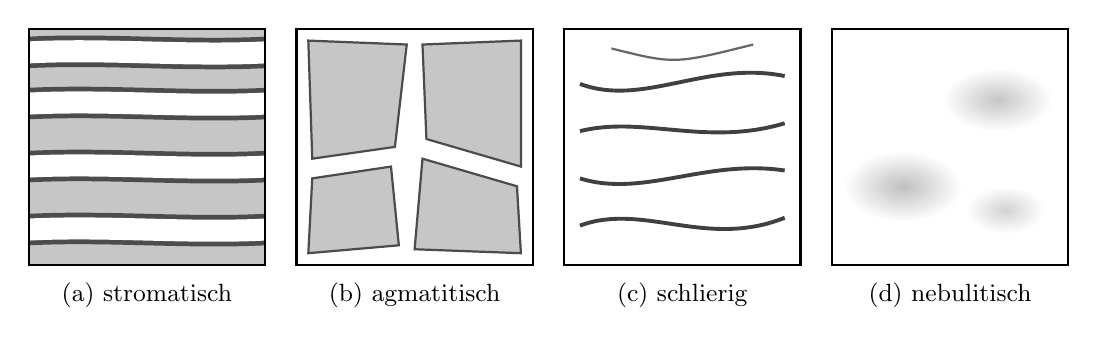
\begin{tikzpicture}[x=1cm, y=1cm]
% (a) stromatic
\begin{scope}
\fill[gray!45] (0,0) rectangle (3,3);
\foreach \y in {0.45, 1.25, 2.05, 2.7} {
  \fill[black!70] (0,\y-0.2) .. controls (1,\y-0.15) and (2,\y-0.25) .. (3,\y-0.2)
    -- (3,\y+0.2) .. controls (2,\y+0.15) and (1,\y+0.25) .. (0,\y+0.2) -- cycle;
  \fill[white] (0,\y-0.14) .. controls (1,\y-0.09) and (2,\y-0.19) .. (3,\y-0.14)
    -- (3,\y+0.14) .. controls (2,\y+0.09) and (1,\y+0.19) .. (0,\y+0.14) -- cycle;
}
\draw[thick] (0,0) rectangle (3,3);
\node[font=\small, anchor=north] at (1.5,-0.1) {(a) stromatisch};
\end{scope}
% (b) agmatitic
\begin{scope}[xshift=3.4cm]
\fill[white] (0,0) rectangle (3,3);
\fill[gray!45, draw=black!70, thick] (0.15,0.15) -- (1.3,0.25) -- (1.2,1.25) -- (0.2,1.1) -- cycle;
\fill[gray!45, draw=black!70, thick] (1.5,0.2) -- (2.85,0.15) -- (2.8,1.0) -- (1.6,1.35) -- cycle;
\fill[gray!45, draw=black!70, thick] (0.2,1.35) -- (1.25,1.5) -- (1.4,2.8) -- (0.15,2.85) -- cycle;
\fill[gray!45, draw=black!70, thick] (1.65,1.6) -- (2.85,1.25) -- (2.85,2.85) -- (1.6,2.8) -- cycle;
\draw[thick] (0,0) rectangle (3,3);
\node[font=\small, anchor=north] at (1.5,-0.1) {(b) agmatitisch};
\end{scope}
% (c) schlieric
\begin{scope}[xshift=6.8cm]
\fill[white] (0,0) rectangle (3,3);
\foreach \y/\a in {0.5/0.3, 1.1/-0.25, 1.7/0.2, 2.3/-0.3} {
  \draw[black!75, line width=1.4pt] (0.2,\y) .. controls (1,\y+\a) and (1.8,\y-\a) .. (2.8,\y+0.1);
}
\draw[black!60, line width=0.8pt] (0.6,2.75) .. controls (1.4,2.55) .. (2.4,2.8);
\draw[thick] (0,0) rectangle (3,3);
\node[font=\small, anchor=north] at (1.5,-0.1) {(c) schlierig};
\end{scope}
% (d) nebulitic
\begin{scope}[xshift=10.2cm]
\fill[white] (0,0) rectangle (3,3);
\shade[inner color=gray!50, outer color=white] (0.9,1.0) ellipse (0.75 and 0.45);
\shade[inner color=gray!45, outer color=white] (2.1,2.1) ellipse (0.7 and 0.4);
\shade[inner color=gray!35, outer color=white] (2.2,0.7) ellipse (0.5 and 0.3);
\draw[thick] (0,0) rectangle (3,3);
\node[font=\small, anchor=north] at (1.5,-0.1) {(d) nebulitisch};
\end{scope}
\end{tikzpicture}
\par\smallskip{\small Vier structuren van \omterm{def:b2:crustal-melting:migmatite}{migmatieten}, schematisch (ontsluitingsvlakken van ongeveer een meter
breed). Wit: \omterm{def:b2:crustal-melting:migmatite}{leucosoom}; zwart: \omterm{def:b2:crustal-melting:migmatite}{melanosoom}; grijs: mesosoom. (a) Stromatisch: lagen
\omterm{def:b2:crustal-melting:migmatite}{leucosoom}, elk met een donkere zoom, evenwijdig aan de foliatie, typisch voor \omterm{def:b2:crustal-melting:migmatite}{metatexieten}.
(b) Agmatitisch: een netwerk van leucosoomaders rond hoekige blokken, met een breccieachtig
uiterlijk. (c) Schlierig: slierten donkere mineralen in het \omterm{def:b2:crustal-melting:migmatite}{leucosoom}. (d) Nebulitisch: vage
schimmen van het vroegere gesteente in een magmatisch ogende gastheer; (c) en (d) zijn typisch voor
\omterm{def:b2:crustal-melting:migmatite}{diatexieten}.}
\end{omfigure}
% ledger: bgs99:migmatite, scmr:migmatite

\begin{omfigure}
\centering
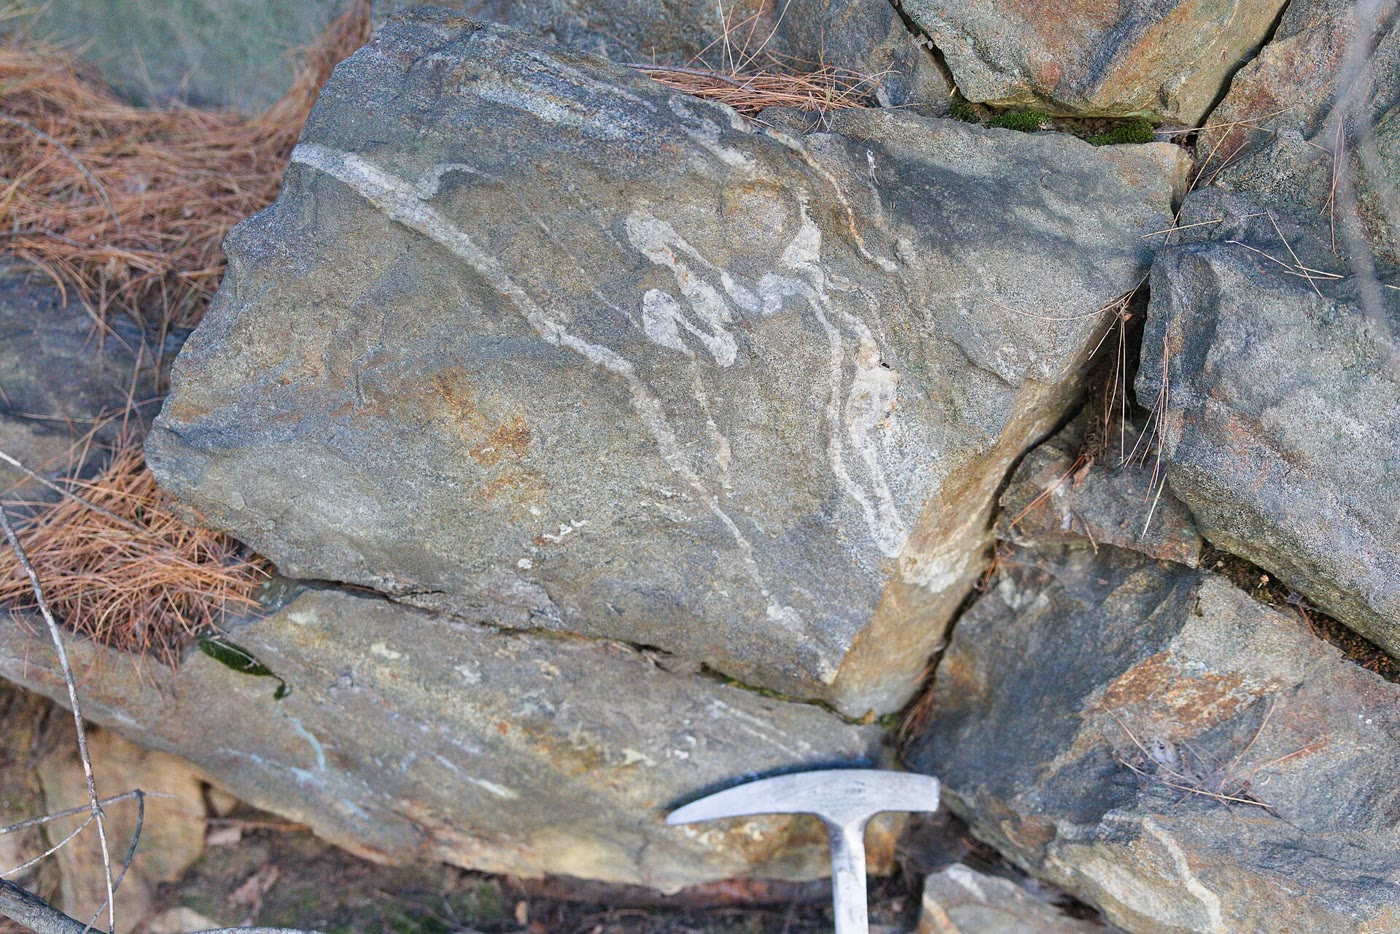
\includegraphics[width=0.62\linewidth]{images/book4/b2-12-migmatite.jpg}
\par\smallskip{\small Een \omterm{def:b2:crustal-melting:migmatite}{migmatiet} in Nashua, New Hampshire: lichte leucosoomaders, geplooid
met de grijze gneis die ze bevat. De geologenhamer geeft de schaal. Foto Kevin M. Gill, CC BY 4.0.}
\end{omfigure}

\section{Van migmatiet naar pluton}\label{sec:b2:crustal-melting:segregation}

Op korrelschaal ligt de eerste smelt langs de korrelgrenzen en in kleine poeltjes,
meestal evenwijdig aan de foliatie. Hoe weinig ook, ze verandert het gesteente: bij experimenten met
partieel gesmolten graniet daalt de sterkte van het aggregaat steil tussen de solidus
en een \omterm{def:b2:mantle-melting:fraction}{smeltfractie} van \num{0.07}, wanneer de smelthoudende korrelgrenzen verbonden raken, en daalt
opnieuw, met ongeveer vier ordes van grootte maar vanaf een al lage waarde, wanneer het
kristalraamwerk bij hogere \omterm{def:b2:mantle-melting:fraction}{smeltfracties} bezwijkt. Partieel gesmolten korst is daarom zwak,
en vervorming concentreert zich daar zodra het smelten begint. Vervorming drijft op haar beurt de
smelt: die loopt uit de matrix weg langs verbonden korrelgrenzen naar \omterm{def:b2:crustal-melting:migmatite}{leucosomen} evenwijdig aan
de foliatie, daarna uit de smeltende laag via \omterm{def:b2:crustal-melting:migmatite}{leucosomen} die haar doorsnijden, en
deze komen samen in de \omterm{def:b2:magma-emplacement:bodies}{gangen} van \cref{ch:b2:magma-emplacement}. De figuur hieronder vat het
pad van de bron tot de \omterm{def:b2:magma-emplacement:bodies}{pluton} samen.
% ledger: sawyer01:segregation, rh05:connectivity

\begin{omfigure}
\centering
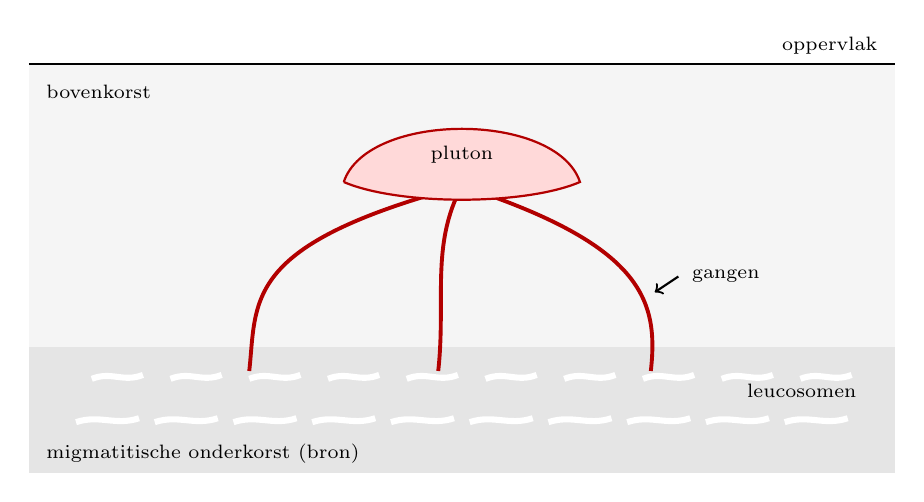
\begin{tikzpicture}[x=1cm, y=1cm]
\fill[gray!20] (0,0) rectangle (11,1.6);
\fill[gray!8] (0,1.6) rectangle (11,5.2);
\node[font=\scriptsize, anchor=west] at (0.1,0.25) {migmatitische onderkorst (bron)};
\foreach \x in {0.6,1.6,2.6,3.6,4.6,5.6,6.6,7.6,8.6,9.6} {
  \draw[white, line width=2.2pt] (\x,0.65) .. controls (\x+0.3,0.75) and (\x+0.5,0.6) .. (\x+0.8,0.7);
  \draw[white, line width=2.2pt] (\x+0.2,1.2) .. controls (\x+0.45,1.3) and (\x+0.6,1.15) .. (\x+0.85,1.25);
}
\foreach \x in {2.8, 5.2, 7.9} {
  \draw[red!70!black, line width=1.4pt] (\x,1.3) .. controls (\x+0.1,2.2) and (\x-0.1,2.9) .. (5.5,3.65);
}
\fill[pink!60, draw=red!70!black, thick] (4.0,3.7) .. controls (4.3,4.6) and (6.7,4.6) .. (7.0,3.7)
  .. controls (6.3,3.4) and (4.7,3.4) .. (4.0,3.7);
\node[font=\scriptsize] at (5.5,4.05) {pluton};
\node[font=\scriptsize, anchor=west] at (8.3,2.5) {gangen};
\draw[->, thick] (8.25,2.5) -- (7.95,2.3);
\node[font=\scriptsize, anchor=west] at (0.1,4.85) {bovenkorst};
\draw[thick] (0,5.2) -- (11,5.2);
\node[font=\scriptsize, anchor=south east] at (10.9,5.2) {oppervlak};
\node[font=\scriptsize, align=left, anchor=west] at (9.0,1.05) {leucosomen};
\end{tikzpicture}
\par\smallskip{\small Van \omterm{def:b2:crustal-melting:migmatite}{migmatiet} naar \omterm{def:b2:magma-emplacement:bodies}{pluton}, schematisch en niet op schaal: \omterm{def:b2:crustal-melting:migmatite}{leucosomen}
(wit) in de partieel gesmolten bron komen samen in \omterm{def:b2:magma-emplacement:bodies}{gangen} (rood) die een \omterm{def:b2:magma-emplacement:bodies}{pluton} hoger in
de korst voeden.}
\end{omfigure}

Hoe lang blijft de korst gesmolten? In de Himalaya begon wijdverbreide \omterm{def:b2:crustal-melting:anatexis}{anatexis} zo'n
30 miljoen jaar na de botsing van India met Azië, en de zirkoon en monaziet van de
anatectische gesteenten geven ouderdommen van ongeveer 25 tot 15 miljoen jaar geleden; één monster kan
het grootste deel van dit interval bestrijken. Het smelten van de korst van de Himalaya was geen gebeurtenis maar een toestand die
ongeveer tien miljoen jaar duurde.
% ledger: weinberg16:himalaya

\section{Graniettypen}\label{sec:b2:crustal-melting:types}

Een graniet onthoudt zijn bron in zijn chemie, in de eerste plaats in hoeveel aluminium het
bevat vergeleken met wat zijn veldspaten kunnen opnemen.

\begin{definition}[Aluminiumverzadigingsindex]\label{def:b2:crustal-melting:asi}
De \emph{aluminiumverzadigingsindex}\index{aluminiumverzadigingsindex} van een gesteente is de
molaire verhouding
\[\mathrm{A/CNK} = \frac{n(\ce{Al2O3})}{n(\ce{CaO}) + n(\ce{Na2O}) + n(\ce{K2O})},\]
en zijn tegenhanger is $\mathrm{A/NK} = n(\ce{Al2O3})/[n(\ce{Na2O}) + n(\ce{K2O})]$. Een gesteente
is \emph{peraluminisch}\index{peraluminisch} als $\mathrm{A/CNK} > 1$,
\emph{metaluminisch}\index{metaluminisch} als $\mathrm{A/CNK} < 1 < \mathrm{A/NK}$, en
\emph{peralkalisch}\index{peralkalisch} als $\mathrm{A/NK} < 1$.
\end{definition}
% ledger: moyen17:aluminosity, frost01:asi

\begin{proposition}[Wat de index meet]\label{prop:b2:crustal-melting:feldspar}
Een gesteente waarvan het calcium, natrium en kalium allemaal in veldspaten zitten, en waarvan het aluminium
helemaal in veldspaten zit, heeft $\mathrm{A/CNK} = 1$. Een \omterm{def:b2:crustal-melting:asi}{peraluminisch} gesteente houdt dus aluminium
over na zijn veldspaten, opgeslagen in aluminiumrijke mineralen (muscoviet, granaat, cordieriet,
aluminiumsilicaat); een \omterm{def:b2:crustal-melting:asi}{metaluminisch} gesteente houdt calcium over, opgeslagen in calciumsilicaten
(hoornblende, clinopyroxeen, titaniet); en een \omterm{def:b2:crustal-melting:asi}{peralkalisch} gesteente houdt natrium en kalium
over, opgeslagen in mineralen zonder genoeg aluminium voor veldspaat (natriumpyroxeen en
natriumamfibool).
\end{proposition}

\begin{proof}
In oxidevorm is kaliveldspaat \ce{K2O.Al2O3.6SiO2}, albiet \ce{Na2O.Al2O3.6SiO2} en
anorthiet \ce{CaO.Al2O3.2SiO2}: elke formule heeft precies één \ce{Al2O3} per
\ce{K2O}, \ce{Na2O} of \ce{CaO}. Elk mengsel van de drie heeft daarom $n(\ce{Al2O3}) =
n(\ce{CaO}) + n(\ce{Na2O}) + n(\ce{K2O})$, dat wil zeggen $\mathrm{A/CNK} = 1$. Als
$\mathrm{A/CNK} > 1$, overtreft het aluminium wat de alkaliën en het calcium in
veldspaat kunnen binden, en moet het overschot in andere mineralen zitten. Als $\mathrm{A/CNK} < 1$ maar
$\mathrm{A/NK} > 1$, is er genoeg aluminium voor al het natrium en kalium als
veldspaat maar niet voor al het calcium, dat terechtkomt in mineralen die minder aluminium
per calcium nodig hebben dan anorthiet. Als $\mathrm{A/NK} < 1$, kunnen zelfs de alkaliën niet allemaal in
veldspaat zitten.
\end{proof}

Moyen en collega's vonden de aluminositeit de nuttigste indicator om granieten
met verschillende bronnen van elkaar te onderscheiden; Frost en collega's gebruiken dezelfde index, met een kleine
correctie voor fosfor, als een van de drie assen van hun classificatie van granitische
gesteenten.
% ledger: moyen17:aluminosity, frost01:asi

\begin{omfigure}
\centering
\begin{tikzpicture}
\begin{axis}[omrecord, width=0.72\linewidth, height=7cm,
  xmin=0.4, xmax=1.5, ymin=0.4, ymax=3.5, xlabel={A/CNK (molair)}, ylabel={A/NK (molair)},
  tick label style={font=\scriptsize}, label style={font=\small}]
\addplot[fill=gray!15, draw=none] coordinates {(0.4,0.4) (1.5,1.5) (1.5,0.4) (0.4,0.4)};
\addplot[thick, black!70] coordinates {(1,0.4) (1,3.5)};
\addplot[thick, black!70] coordinates {(0.4,1) (1.5,1)};
\node[font=\scriptsize, anchor=north east] at (axis cs:1.48,3.45) {peraluminisch};
\node[font=\scriptsize, anchor=west] at (axis cs:0.62,2.6) {metaluminisch};
\node[font=\scriptsize, anchor=south west] at (axis cs:0.42,0.45) {peralkalisch};
\addplot[only marks, mark=*, mark size=2pt, blue!70!black, nodes near coords,
  point meta=explicit symbolic, every node near coord/.style={font=\scriptsize, anchor=west}]
  coordinates {(0.539,3.196)[BHVO-2] (0.877,1.694)[AGV-2] (0.993,1.135)[SRM 278]};
\addplot[only marks, mark=square*, mark size=2pt, red!70!black]
  coordinates {(1.261,1.377) (0.809,0.844)};
\node[font=\scriptsize, red!70!black, anchor=south] at (axis cs:1.261,1.45) {smelt van S-type};
\node[font=\scriptsize, red!70!black, anchor=north] at (axis cs:0.809,0.79) {peralkalisch graniet};
\end{axis}
\end{tikzpicture}
\par\smallskip{\small Het diagram van Shand. Blauwe cirkels: drie referentiematerialen, een Hawaïaanse
basalt (BHVO-2), een andesiet (AGV-2) en een obsidiaan met granitische samenstelling (SRM 278),
berekend uit hun gepubliceerde oxidegehalten. Rode vierkanten: twee verzonnen granieten die in
dit hoofdstuk worden gebruikt. De grijze driehoek is onbereikbaar, omdat A/CNK nooit groter is dan A/NK.}
\end{omfigure}
% ledger: usgs:bhvo2-major, usgs:agv2-major, nist278:majors

De chemie volgt de bron. In 1974 merkten Chappell en White op dat de granieten van de Lachlan Fold Belt, op de
meest felsische gesteenten na, in twee duidelijke groepen uiteenvallen,
en ze interpreteerden die als smelten van twee soorten brongesteente: oudere stollingsgesteenten en sedimentgesteenten. De hydrolyse van veldspaten (zie Boek~3)
voert natrium en calcium in oplossing af en houdt aluminium vast in kleien: modder die
uit deze kleien bestaat, is rijk aan aluminium, en hun smelten ook.
% ledger: cw01:is-types

\begin{definition}[Graniettypologie]\label{def:b2:crustal-melting:types}
Een \emph{graniet van I-type}\index{graniet van I-type} is een graniet waarvan de bron overwegend een
ouder stollingsgesteente was, een \emph{graniet van S-type}\index{graniet van S-type} een graniet waarvan de bron
overwegend een sedimentair (metasedimentair) gesteente was, en een graniet van M-type een graniet afkomstig uit
de mantel. Een \emph{graniet van A-type}\index{graniet van A-type} wordt gedefinieerd door zijn chemie en
omgeving, niet door zijn bron: ijzerrijk en kaliumrijk, sterk verrijkt in \omterm{def:b2:elements-in-the-earth:partition}{incompatibele
elementen}, en geplaatst in stabiele intraplaat-, backarc- of postcollisionele omgevingen.
\end{definition}
% ledger: johansson23:a-type, cw01:is-types

Granieten van S-type zijn \omterm{def:b2:crustal-melting:asi}{peraluminisch}, met twee mica's of met cordieriet; granitoïden van A-type
zijn meestal \omterm{def:b2:crustal-melting:asi}{metaluminisch}, sommige \omterm{def:b2:crustal-melting:asi}{peraluminisch}. Eén analyse kan echter misleiden: elke
granitoïdreeks eindigt dicht bij de samenstelling van het granitische minimum, leucocraat en zwak
\omterm{def:b2:crustal-melting:asi}{peraluminisch}, zodat een \omterm{def:b2:crustal-melting:asi}{peraluminisch} monster geen bewijs is dat korst gesmolten werd. Wat
reeksen van elkaar onderscheidt, is de vorm van hun trend in het diagram van Shand: een boogreeks bereikt het
minimum langs een steile reeks punten vanaf hoge A/NK en lage A/CNK, een calciumarme reeks van S-type
langs een reeks punten met A/NK dicht bij A/CNK. Over de bron van de \omterm{def:b2:magma-emplacement:magma}{magma's} van A-type
is geen consensus bereikt: één model maakt ze uit basalt van onderplating, geëvolueerd door kristallisatie,
\omterm{def:b2:mantle-melting:melting}{partieel smelten} en assimilatie van korst.
% ledger: moyen17:trends, frost01:asi, johansson23:a-type

\begin{definition}[Leucograniet]\label{def:b2:crustal-melting:leucogranite}
Een \emph{leucograniet}\index{leucograniet} is een lichtgekleurd graniet, bijna vrij van
donkere mineralen; de peraluminische leucogranieten van botsingsgordels bevatten muscoviet, alleen of
met biotiet.
\end{definition}
% ledger: moyen17:aluminosity, pdh98:himalaya

De muscoviethoudende peraluminische \omterm{def:b2:crustal-melting:leucogranite}{leucogranieten} van botsingsgordels hebben samenstellingen die dicht
bij de vloeistoffen van smelten met water of \omterm{def:b2:crustal-melting:reactions}{dehydratatiesmelten} van muscoviet liggen, bij temperaturen rond
\qty{700}{\celsius} waarbij zirkoon en monaziet van de bron kunnen overleven en als
xenokristen in de smelt worden meegevoerd; cordieriethoudende peraluminische granieten komen van het
hetere uiteenvallen van biotiet, bij 800 tot \qty{850}{\celsius}. De \omterm{def:b2:crustal-melting:leucogranite}{leucogranieten} van de Himalaya,
met hun sterke isotopische signatuur van de korst, behoren tot deze familie
(\cref{ch:b2:himalaya-andes}).
% ledger: moyen17:aluminosity, weinberg16:himalaya

\begin{omfigure}
\centering
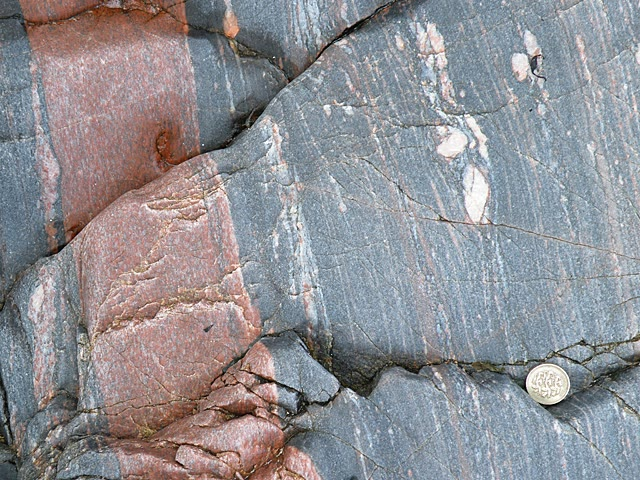
\includegraphics[width=0.5\linewidth]{images/book4/b2-12-leucogranite-vein.jpg}
\par\smallskip{\small Een roze leucograniet-ader die een gebande grijze gneis doorsnijdt; de munt geeft
de schaal. Foto Anne Burgess (Geograph), CC BY-SA 2.0.}
\end{omfigure}

\section{Granieten en de groei van de continenten}\label{sec:b2:crustal-melting:time}

Twee soorten plaatsen maken het meeste graniet. Boven subductiezones vormt boogkorst zich door de
differentiatie van mafische smelten uit de mantel, en de beschikbare warmte is alleen wat deze
smelten meebrengen. Na een botsing is de verdikte korst een zeer heet systeem: ze smelt op
grote schaal, bij lage temperatuur waar water of muscoviet het toelaat en bij hogere
temperatuur door het uiteenvallen van biotiet, en deze uit de korst afkomstige granieten recyclen korst die
al bestond. Ook daar bereiken mantelsmelten de korst, in hoeveelheden die groot genoeg zijn, zo betogen Moyen en
collega's, om laatorogene gordels tot belangrijke bijdragers aan de groei van de
korst te maken. Of een graniet iets toevoegt aan de continenten of ze alleen herwerkt, is dus een vraag naar
zijn bron, die zijn isotopen beantwoorden (\cref{ch:b2:isotope-geochemistry}); de granieten van
de vroege Aarde, heel anders dan deze, zijn het onderwerp van
\cref{ch:b2:precambrian-earth}.
% ledger: moyen17:settings

\section{Oefeningen}\label{sec:b2:crustal-melting:exercises}

Molaire massa's (\unit{\gram\per\mole}): \ce{Al2O3} 101.96, \ce{CaO} 56.08, \ce{Na2O} 61.98,
\ce{K2O} 94.20, \ce{H2O} 18.02; atoommassa's: H 1.008, O 16.00, Na 22.99, Mg 24.31,
Al 26.98, Si 28.09, K 39.10, Ca 40.08. Neem $g = \qty{9.81}{\metre\per\second\squared}$.

\begin{exercise}[$\star$]\label{exo:b2:crustal-melting:1}
Het referentiemateriaal AGV-2, een andesiet, bevat in \unit{\gram} per \qty{100}{\gram}
\ce{Al2O3} 17.03, \ce{CaO} 5.15, \ce{Na2O} 4.204 en \ce{K2O} 2.898.
(a) Bereken zijn A/CNK en A/NK. (b) Classificeer het, en noem een mineraal dat zijn
overtollige calcium zou moeten bevatten.
\end{exercise}
% ledger: usgs:agv2-major

\begin{exercise}[$\star$]\label{exo:b2:crustal-melting:2}
Drie granieten bevatten, naast kwarts en veldspaten: (a) muscoviet, biotiet en granaat;
(b) hoornblende, biotiet en titaniet; (c) aegirien, een natrium-ijzerpyroxeen
\ce{NaFeSi2O6}, en een natriumamfibool. Classificeer elk naar zijn aluminiumverzadiging, en zeg
welk een \omterm{def:b2:crustal-melting:types}{graniet van S-type} zou kunnen zijn.
\end{exercise}

\begin{exercise}[$\star$]\label{exo:b2:crustal-melting:3}
Een korst met dichtheid \qty{2800}{\kilogram\per\cubic\metre} heeft een lineaire geotherm
$T = \qty{10}{\celsius} + (\qty{20}{\celsius\per\kilo\metre})\,z$. Benader tussen 2 en
\qty{10}{kbar} de natte granietsolidus door de rechte lijn door
(\qty{680}{\celsius}, \qty{2}{kbar}) en (\qty{620}{\celsius}, \qty{10}{kbar}). Op welke
diepte, temperatuur en druk snijdt de geotherm haar?
\end{exercise}
% ledger: sw81:wet-solidus

\begin{exercise}[$\star$]\label{exo:b2:crustal-melting:4}
Een grijze biotietgneis bevat centimeterdikke witte lagen van kwarts en veldspaat, evenwijdig
aan zijn foliatie, elk omzoomd door een dunne zwarte naad van biotiet; tussen de lagen ziet de
gneis er gewoon uit. (a) Benoem de witte lagen, de zwarte naden en de gewone gneis.
(b) Is het gesteente een \omterm{def:b2:crustal-melting:migmatite}{metatexiet} of een \omterm{def:b2:crustal-melting:migmatite}{diatexiet}, en wat is zijn structuur? (c) Een paar honderd
meter verderop is de gelaagdheid verdwenen: een slierig, granietachtig gesteente bevat vage schimmen van
gneis. Wat is er veranderd?
\end{exercise}
% ledger: scmr:migmatite, bgs99:migmatite

\begin{exercise}[$\star\star$]\label{exo:b2:crustal-melting:5}
Neem biotiet als flogopiet, \ce{KMg3AlSi3O10(OH)2}. (a) Bereken zijn molaire massa en de
massafractie water die het afgeeft (zijn twee hydroxylgroepen geven één \ce{H2O}).
(b) Een gneis met \qty{25}{\percent} biotiet in massa smelt door \omterm{def:b2:crustal-melting:reactions}{dehydratatiesmelten} van biotiet
tot een smelt met \qty{4.0}{\percent} water. Bepaal met
\cref{prop:b2:crustal-melting:water} de \omterm{def:b2:mantle-melting:fraction}{smeltfractie}, en vergelijk die met de
fracties die bij experimenten met \omterm{def:b2:crustal-melting:reactions}{dehydratatiesmelten} van biotiet werden gevonden.
\end{exercise}
% ledger: bk99:migmatites

\begin{exercise}[$\star\star$]\label{exo:b2:crustal-melting:6}
Honderd gram graniet bevat \qty{30}{\gram} kaliveldspaat \ce{KAlSi3O8},
\qty{35}{\gram} albiet \ce{NaAlSi3O8}, \qty{5}{\gram} anorthiet \ce{CaAl2Si2O8},
\qty{25}{\gram} kwarts en \qty{5}{\gram} muscoviet \ce{KAl3Si3O10(OH)2}.
(a) Bereken de molaire massa's van de vier aluminiumhoudende mineralen. (b) Bereken de hoeveelheden
\ce{Al2O3}, \ce{CaO}, \ce{Na2O} en \ce{K2O} in het gesteente, en zijn A/CNK. (c) Welk
mineraal maakt het gesteente \omterm{def:b2:crustal-melting:asi}{peraluminisch}?
\end{exercise}

\begin{exercise}[$\star\star$]\label{exo:b2:crustal-melting:7}
Een basaltische \omterm{def:b2:magma-emplacement:bodies}{sill}, geïntrudeerd bij \qty{1200}{\celsius}, kristalliseert volledig en koelt af tot
\qty{850}{\celsius}, waarbij een latente warmte van \qty{900}{\mega\joule\per\cubic\metre} vrijkomt.
De korst eromheen, op \qty{650}{\celsius}, wordt verhit tot \qty{850}{\celsius} en
\qty{20}{\percent} ervan smelt, met dezelfde latente warmte per volume-eenheid smelt. Beide
gesteenten hebben een warmtecapaciteit van \qty{2.5}{\mega\joule\per\cubic\metre\per\kelvin}. Hoeveel kubieke meter
korst kan, volgens \cref{prop:b2:crustal-melting:heat}, één kubieke meter
basalt zo behandelen? Wat verwaarloost het resultaat?
\end{exercise}
% ledger: delaney86b4:properties

\begin{exercise}[$\star\star$]\label{exo:b2:crustal-melting:8}
Het obsidiaan-referentiemateriaal SRM 278 is gecertificeerd op \ce{Al2O3}
$14.15 \pm 0.15$, \ce{CaO} 0.983, \ce{Na2O} 4.84 en \ce{K2O} 4.16 (\unit{\percent} in
massa). (a) Bereken zijn A/CNK en A/NK en classificeer het. (b) Bereken A/CNK opnieuw met de twee
uitersten van de onzekerheid op \ce{Al2O3}. Is de classificatie robuust?
\end{exercise}
% ledger: nist278:majors

\begin{exercise}[$\star\star$]\label{exo:b2:crustal-melting:9}
Bij \qty{800}{\celsius} bevat een met water verzadigde haplogranietsmelt \qty{7.45}{\percent}
water bij \qty{3}{kbar}, 8.94 bij \qty{4}{kbar}, 9.97 bij \qty{5}{kbar} en 13.82 bij
\qty{8}{kbar}. (a) Pas met de kleinstekwadratenmethode een rechte lijn aan deze vier punten aan en vergelijk
haar helling met de \qty{1.27}{\percent} per kilobar die de experimentatoren opgeven.
(b) Voorspel het verzadigingsgehalte bij \qty{6}{kbar}. (c) Wat is de kleinste massa smelt
die \qty{10}{\gram} water kan meevoeren bij \qty{6}{kbar}? (d) Waarom mag de lijn niet
worden gebruikt bij \qty{15}{kbar}?
\end{exercise}
% ledger: holtz95:solubility

\begin{exercise}[$\star\star\star$]\label{exo:b2:crustal-melting:10}
Benader de solidus van het \omterm{def:b2:crustal-melting:reactions}{dehydratatiesmelten} van een muscovietschist door de rechte lijn
door (\qty{750}{\celsius}, \qty{6}{kbar}) en (\qty{800}{\celsius}, \qty{10}{kbar}),
de uiteinden van de experimentele intervallen. Een schist op \qty{770}{\celsius} stijgt op vanaf
\qty{10}{kbar} zonder warmte op te nemen of te verliezen. (a) Bij welke druk bereikt hij de
solidus? (b) Daarna volgt zijn temperatuur de solidus omlaag, en de warmte voor het smelten komt
uit zijn eigen afkoeling. Neem een warmtecapaciteit van \qty{2.5}{\mega\joule\per\cubic\metre\per\kelvin}
en een latente warmte van \qty{900}{\mega\joule\per\cubic\metre}: welke volumefractie smelt
is er gevormd wanneer hij \qty{6}{kbar} bereikt? (c) Vergelijk met de omstandigheden die voor de
\omterm{def:b2:crustal-melting:leucogranite}{leucogranieten} van de Himalaya zijn voorgesteld.
\end{exercise}
% ledger: pdh98:himalaya, delaney86b4:properties

\begin{exercise}[$\star\star\star$]\label{exo:b2:crustal-melting:11}
Warmte diffundeert over een afstand $\ell$ in een tijd van de orde $\ell^2/\kappa$. Schat met
$\kappa = \qty{1e-6}{\square\metre\per\second}$ de tijd die de warmte van een
\qty{2}{km} dikke \omterm{def:b2:magma-emplacement:bodies}{sill}, en van een \qty{10}{km} dikke laag van onderplating, nodig heeft om zich over haar
eigen dikte te verspreiden. Vergelijk met de tien miljoen jaar van \omterm{def:b2:crustal-melting:anatexis}{anatexis} in de Himalaya: kan één
onderplatingsgebeurtenis die verklaren?
\end{exercise}
% ledger: delaney86b4:properties, weinberg16:himalaya

\begin{exercise}[$\star\star\star$]\label{exo:b2:crustal-melting:12}
Een stromatisch \omterm{def:b2:crustal-melting:migmatite}{migmatiet} wordt geanalyseerd: \omterm{def:b2:crustal-melting:migmatite}{leucosoom} \ce{K2O} \qty{5.0}{\percent}, \ce{MgO}
\qty{0.20}{\percent}; \omterm{def:b2:crustal-melting:migmatite}{melanosoom} \ce{K2O} \qty{2.0}{\percent}, \ce{MgO}
\qty{4.0}{\percent}; mesosoom, beschouwd als het ongesmolten moedergesteente, \ce{K2O}
\qty{2.75}{\percent}, \ce{MgO} \qty{3.05}{\percent} (alles in massa). (a) Als het
neosoom zonder winst of verlies uit het moedergesteente ontstond, welke massafractie ervan is
\omterm{def:b2:crustal-melting:migmatite}{leucosoom}? (b) Controleer het antwoord met \ce{MgO}. (c) Op de ontsluiting maakt het \omterm{def:b2:crustal-melting:migmatite}{leucosoom} slechts
\qty{10}{\percent} van het neosoom in massa uit. Hoeveel gram smelt vertrok per
\qty{100}{\gram} moedergesteente?
\end{exercise}

\begin{problem}[{Weekendprobleem --- een pluton uit gesmolten mica}]\label{pb:b2:crustal-melting:1}
Een schist uit \qty{20}{\percent} muscoviet, \qty{15}{\percent} biotiet,
\qty{30}{\percent} kwarts, \qty{30}{\percent} plagioklaas en \qty{5}{\percent} andere
mineralen (in massa; een verzonnen gesteente) ligt aan de basis van een korst die door stapeling is verdubbeld, de
situatie die in \cref{ch:b2:pt-paths} is gemodelleerd. Hij kan smelten en een granietpluton voeden. Gegevens:
de atoom- en molaire massa's aan het begin van de oefeningen; de natte granietsolidus gaat
door (\qty{680}{\celsius}, \qty{2}{kbar}), (\qty{620}{\celsius}, \qty{10}{kbar}),
(\qty{605}{\celsius}, \qty{15.3}{kbar}) en (\qty{670}{\celsius}, \qty{27}{kbar}); het
waterverzadigingsgehalte van een granitische smelt bij \qty{800}{\celsius} is \qty{9.97}{\percent} bij
\qty{5}{kbar} en \qty{13.82}{\percent} bij \qty{8}{kbar}. De modelbasis van de verdikte korst volgt dit verloop:

\smallskip
\begin{center}\small
\begin{tabular}{l|ccccccccccc}
$t$ (\unit{Myr}) & 0 & 10 & 20 & 30 & 40 & 50 & 60 & 70 & 80 & 90 & 100\\ \hline
$T$ (\unit{\celsius}) & 595 & 656 & 734 & 795 & 845 & 885 & 909 & 914 & 900 & 867 & 814\\
$P$ (\unit{kbar}) & 19.2 & 19.2 & 19.2 & 19.2 & 17.9 & 16.5 & 15.1 & 13.7 & 12.4 & 11.0 & 9.6
\end{tabular}
\end{center}
\smallskip

\noindent\textbf{Deel I --- Water uit mica.}
\begin{enumerate}
\item Bereken de molaire massa van muscoviet \ce{KAl3Si3O10(OH)2}.
\item Zijn twee hydroxylgroepen geven één \ce{H2O}. Welke massafractie van het mineraal
komt vrij als water?
\item Hoeveel water geeft de muscoviet van één kilogram schist af?
\item Wat is, bij lineaire interpolatie, het verzadigingswatergehalte van de smelt bij
\qty{7}{kbar}? Wat is dan de kleinste \omterm{def:b2:mantle-melting:fraction}{smeltfractie} die het water van de muscoviet kan maken?
\item De smelt van \omterm{def:b2:crustal-melting:reactions}{dehydratatiesmelten} is verre van verzadigd; neem zijn watergehalte
\qty{6.0}{\percent}. Welke \omterm{def:b2:mantle-melting:fraction}{smeltfractie} maakt de muscoviet?
\item Bij experimenten met een \omterm{def:b2:metamorphic-facies:protoliths}{metapeliet} met twee mica's bij \qty{10}{kbar} gaf de muscovietreactie
slechts 1 tot \qty{2}{\percent} smelt. Noem twee redenen waarom een echt gesteente minder
smelt kan maken dan het antwoord op vraag~5.
\end{enumerate}

\noindent\textbf{Deel II --- De bron verhitten.}
\begin{enumerate}[resume]
\item In \cref{ch:b2:pt-paths} piekt het gesteente dat op middendiepte achterbleef op \qty{593}{\celsius}
en \qty{7.8}{kbar}. Wat is de natte solidus bij \qty{7.8}{kbar}? Kan dat gesteente smelten, zelfs
met vrij water?
\item Bepaal door interpolatie tussen 15.3 en \qty{27}{kbar} de natte solidus bij de druk
van de basis vlak na het stapelen. Ligt de basis erboven bij $t = 0$? Bij $t = \qty{10}{Myr}$?
\item Wat begrenst het smelten van de basis bij $t = \qty{10}{Myr}$, en waarom stopt het
snel?
\item Wanneer passeert de basis \qty{800}{\celsius}, de bovengrens van het
muscovietinterval?
\item Het amfiboolinterval loopt van 875 tot \qty{925}{\celsius} bij 10 tot \qty{12.5}{kbar}.
Wanneer komt de basis in dit drukbereik, en bij welke temperatuur?
\item Wanneer bereikt de basis \qty{10}{kbar}, de bovenkant van het drukbereik van de
muscovietexperimenten, en hoe heet is ze dan? Welke waterhoudende mineralen van de schist kunnen
nog bestaan?
\end{enumerate}

\noindent\textbf{Deel III --- Welke smelt?}
De smelt geeft na kristallisatie een \omterm{def:b2:crustal-melting:leucogranite}{leucograniet} (verzonnen analyse) met, in
\unit{\percent} van de massa, \ce{Al2O3} 15.0, \ce{CaO} 0.55, \ce{Na2O} 3.4 en \ce{K2O} 4.9.
\begin{enumerate}[resume]
\item Bereken de hoeveelheden van de vier oxiden in \qty{100}{\gram} van het gesteente.
\item Bereken zijn A/CNK.
\item Bereken zijn A/NK en classificeer de \omterm{def:b2:crustal-melting:leucogranite}{leucograniet}.
\item Is het een \omterm{def:b2:crustal-melting:types}{graniet van I-type} of van S-type? Noem twee mineralen die zijn overtollige
aluminium zouden moeten bevatten.
\item Hoeveel mol \ce{Al2O3} per \qty{100}{\gram} blijft er over na de
veldspaten? Als dat allemaal in muscoviet ging, dat per formule-eenheid één \ce{Al2O3} meer
bevat dan kaliveldspaat, hoeveel gram muscoviet zou \qty{100}{\gram} graniet dan
bevatten?
\item Het obsidiaan SRM 278 heeft A/CNK $= 0.993$. Kunnen de \omterm{def:b2:crustal-melting:leucogranite}{leucograniet} en het obsidiaan
uit dezelfde soort bron komen?
\end{enumerate}

\noindent\textbf{Deel IV --- Hoeveel korst?}
Een verzonnen \omterm{def:b2:magma-emplacement:bodies}{pluton} van deze \omterm{def:b2:crustal-melting:leucogranite}{leucograniet} heeft een volume van \qty{1000}{\cubic\kilo\metre}.
Neem \qty{2650}{\kilogram\per\cubic\metre} voor het graniet en
\qty{2800}{\kilogram\per\cubic\metre} voor de schist; veronderstel dat \qty{70}{\percent} van de
smelt zijn bron verlaat en dat al het water van de smelt ontsnapt wanneer die kristalliseert.
\begin{enumerate}[resume]
\item Wat is de massa van de \omterm{def:b2:magma-emplacement:bodies}{pluton}?
\item Welke massa smelt (met zijn \qty{6.0}{\percent} water) was ervoor nodig?
\item Welke massa schist moest smelten, met de \omterm{def:b2:mantle-melting:fraction}{smeltfractie} van vraag~5?
\item Welk volume schist is dat?
\item Als de bron een laag van \qty{5}{km} dik was, over welke oppervlakte smolt ze dan?
\item Hoeveel groter zou de bron zijn met in plaats daarvan de kleinste \omterm{def:b2:mantle-melting:fraction}{smeltfractie} van vraag~4? Geef het volume
bronkorst dat werd gesmolten om de \omterm{def:b2:magma-emplacement:bodies}{pluton} te maken, in
\unit{\cubic\kilo\metre}, op basis van vraag~22.
\end{enumerate}
\end{problem}
